
\documentclass[11pt]{article}

\usepackage{fullpage,epsfig,latexsym,picinpar,amsbsy,amsmath}
\usepackage{algorithm}
\usepackage[noend]{algpseudocode}
\usepackage{xspace}

\newcommand{\delete}{{\mbox{\tt delete}}}
\newcommand{\decreasekey}{{\mbox{\tt decreasekey}}}
\newcommand{\extractmin}{{\mbox{\tt extractmin}}}
\newcommand{\level}{{\mbox{\it level}}}


\setlength{\evensidemargin}{0.1in}
\setlength{\oddsidemargin}{0.1in}
\setlength{\textwidth}{6.6in}
\setlength{\topmargin}{0.0in}
\setlength{\textheight}{8.7in}
\setlength{\headheight}{0in}
\setlength{\headsep}{0in}
\setlength{\topsep}{0in}
\setlength{\itemsep}{0in}
\renewcommand{\baselinestretch}{1.1}
\parskip=0.080in
                                                                                                                         
\newcommand{\parend}[1]{{\left( #1  \right) }}
\newcommand{\spparend}[1]{{\left(\, #1  \,\right) }}
\newcommand{\angled}[1]{{\left\langle #1  \right\rangle }}
\newcommand{\brackd}[1]{{\left[ #1  \right] }}
\newcommand{\spbrackd}[1]{{\left[\, #1  \,\right] }}
\newcommand{\braced}[1]{{\left\{ #1  \right\} }}
\newcommand{\leftbraced}[1]{{\left\{ #1  \right. }}
\newcommand{\floor}[1]{{\left\lfloor #1\right\rfloor}}
\newcommand{\ceiling}[1]{{\left\lceil #1\right\rceil}}
\newcommand{\barred}[1]{{\left|#1\right|}}
\newcommand{\doublebarred}[1]{{\left|\left|#1\right|\right|}}
\newcommand{\spaced}[1]{{\, #1\, }}
\newcommand{\suchthat}{{\spaced{|}}}
\newcommand{\numof}{{\sharp}}
\newcommand{\assign}{{\,\leftarrow\,}}
                                                                                                                         
\newcommand{\veps}{{\varepsilon}}
\newcommand{\Sigmastar}{{\Sigma^\ast}}
\newcommand{\barx}{{ \bar x}}

\newcommand{\half}{{\mbox{$\frac{1}{2}$}}}
\newcommand{\threehalfs}{{\mbox{$\frac{3}{2}$}}}





\pagestyle{empty}
\begin{document}

\centerline{\large \bf CS218 ASSIGNMENT 1}
\centerline{due Thursday, January~24 at 5PM}

\vskip 0.1in
\noindent
{\bf Individual assignment: Problems 1,2}

\noindent
{\bf Group assignment: Problems 1,2,3}

\vskip 0.1in

%%%%%%%%%%%%%%%%%%%%%%%%%%%%

\begin{problem} 
(a)
We have a collection of integer variables $x_1,x_2,x_3, ...$,
each with initial value $0$.
We execute a sequence of $n$ operations, where each
operation is either $x_i \assign x_i+1$ (increment)
or $x_i \assign x_i + x_j$ (addition),
for some $i\neq j$. We measure the cost by the number of
bit changes (as in incrementing the binary counter).
Determine the (asymptotic) amortized cost for the operations
of increment and addition.

(b) 
Suppose now that we modify the above problem by adding the
following assumption: after executing an operation
$x_i \assign x_i + x_j$, the variable $x_j$ is ``destroyed" and
cannot be used anymore.
Determine the (asymptotic) amortized costs of
increments and additions with this modification.

You need to give a full justification for your answers.
\end{problem}

\paragraph{Answer}
(a)
For case $x_i \assign x_i+1$, 
The increment cost of $x_i \assign x_i+1$ is $O(1 + number\: of\: trailing\: 1s)$.\\
The amortized cost of increment: $\hat c_k = c_k + \Phi(D_k) - \Phi(D_{k-1})$, where $c_k$ is the actual change of bits, $\Phi(D_k) = $the number of 1s in $x_i$. For example,\\
$x_i = 0000$, $x_i \assign x_i + 1$, $x_i \assign 0001$: $\hat c_k = c_k + \Phi(D_k) + \Phi(D_{i-k}) = 1 + 1 - 0 = 2$.\\
The total amortize cost of increment is $O(n).$

The worst case of a single addition step is that we need to flip all the bits in $x_i$. For example, $x_i=0000, x_j=1111, x_i \assign x_i+x_j = 1111$. If we want to flip the number of bits as much as possible, after every addition, we can get a constant number of 1's more than the last state. Then the total number of 1's in the collection has a $O(n^2)$ cost.\\
We can observe that the actual cost of addition is at most the number of 1's in $x_j$. Then the potential function should be like this:\\
 $\hat c_k = c_k + \Phi(D_k) - \Phi(D_{k-1})$, where $c_k$ is the actual change of bits, $\Phi(D_k) = $the number of 1s in $x_i$ since the change of $x_i$ is the only reason to the total bits change of 1's in the entire collection.\\
$\hat c_k = c_k + \Phi(D_k) - \Phi(D_{k-1}) \leq (number\: of\: 1's\: in\: x_{j_k}) + (number\: of\: 1's\: in\: x_{i_k}) - (number\: of\: 1's\: in\: x_{i_{k-1}})$.\\
Suppose that we operate $y$ times addition to the collection, $n-y$ times increment. After all the operations, the number of 1's will be at most $n^2$ in the integer collection.\\
$\sum\limits_{k=1}^n \hat c_k = \sum\limits_{k=1}^y (number\: of\: 1's\: in\: x_{j_k}) + (number\: of\: 1's\: in\: x_{i_{final}}) \leq n^2$.\\
The total cost of addition is $O(n*b)$, and the amortized cost of addition is $O(n^2)$. The amortized cost of operation is $O(n)$.

(b)
In this case, the state change is the subtraction of changed bits in $x_i$ and the number of bits in $x_j$.
The amortized cost of increment: $\hat c_k = c_k + \Phi(D_k) - \Phi(D_{k-1})$, where $c_k$ is the actual change of bits, $\Phi(D_k) = $the number of 1s in the collection.
\begin{gather*}
    \hat c_k = c_k + \Phi(D_k) - \Phi(D_{k-1}) \\
    \leq (number\: of\: 1's\: in\: x_{j_k}) + (number\: of\: 1's\: in\: x_{i_k}) - (number\: of\: 1's\: in\: x_{i_{k-1}}) - (number\: of\: 1's\: in\: x_{j_k})\\
    \sum\limits_{k=1}^n \hat c_k = (number\: of\: 1's\: in\: x_{i_{final}}) \leq n
\end{gather*}

The total cost of addition is $O(n)$, and the amortized cost of addition is $O(1)$. The amortized cost of operation is $O(1)$.\\

%%%%%%%%%%%%%%%%%%%%%%%%%%%%
\newcommand{\randomkey}{\textit{randomkey}} 
\newcommand{\randomint}{\textit{rand}} 
\newcommand{\union}{\textit{union}} 

\begin{problem}
For a given set $Q$ of keys, let $\randomkey(Q)$ be an operation that generates
a random key from $Q$ (with uniform distribution). For example, if 
$Q = \{4,8,1,2,5\}$, then after executing $k \assign\randomkey(Q)$, the
value of $k$ will be one of the numbers $4,8,1,2,5$, each with probability $\frac{1}{5}$.

Modify Fibonacci heaps to design a data structure that 
%
\begin{description}
	\item{(i)} can perform all priority queue operations
(as defined in class) except $\union()$, in the same amortized time as Fibonacci heaps, and 
	\item{(ii)} in worst-case time $O(1)$ can perform operation
	$\randomkey(Q)$, where $Q$ is the set of keys in the priority queue. 
\end{description}

To clarify, when we say ``except $\union()$'', it means that the data structure will
never be used to execute union operations of different priority queues.
The algorithm for the union operation is still implicit in the implementation of the
$\extractmin()$ operation.

You can assume that you are given a function $\randomint(m)$ that
generates a random number from $1,2,...,m$, each with the same probability.  

You can describe the design of your data structure in words. Illustrate the design
with a figure. (Either a general idea behind your data structure, or an explicit example.)
The implementation of  $\randomkey(Q)$ needs to be described in pseudo-code.
Justify the running time.

\end{problem}

\let\oldReturn\Return
\renewcommand{\Return}{\State\oldReturn}

\paragraph{Answer}
We can keep a hash table to record the already generated numbers. In this way, the average and amortized time complexity of $search()$ operation is $O(1)$.
Every time we use $rand()$ operation to generate a number, we also store the number in the hash table. On the next we call $rand()$ operation to generate a new number, we look it up in the hash table first. If it exists in the hash table, we re-generate a number; if it's not, we keep it, and save a copy into the hash table. The index of the key has been obtained from the above operations, then we need $randomKey()$ to return the key in the data structure.

\begin{algorithm}
\caption{$Random Key$}
\begin{algorithmic}[1]
\Function{randomKey}{$Q[\;]$}
\Procedure{Generating Random Index}{}
\State $\textit{m} \gets \text{length of } \textit{Q}$
\State $\text{create an array } \textit{P[1,...,m], P[k] = k}$
\State $\text{create a hash table } \textit{H}$
\For{$i \gets 1$ to $m$}
    \State $\textit{idx} \gets$ $rand(m)$
    \If{$\textit{H}.\texttt{contiansKey}(\textit{idx}\texttt{)} \text{ is True}$}
        \State $i--$
        \State $\text{continue}$
    \Else
        \State $\textit{H}.\texttt{insertKey}(\textit{idx}\texttt{)}$
    \EndIf
\EndFor
\EndProcedure
\Procedure{Find in the Data Structure}{}
\State $\text{Store the data structure as a list }\textit{DS[\;]}$
\Return $\textit{DS[idx]}$
\EndProcedure
\EndFunction
\end{algorithmic}
\end{algorithm}

\newpage
%%%%%%%%%%%%%%%%%%%%%%%%%%%%

\begin{problem} 
The figure below shows a transition diagram with costs on transitions,
similar to the example we discussed in class.
Determine the amortized cost of traversing this graph.
You can assume that $A$ is the initial state.

\noindent
\begin{center}
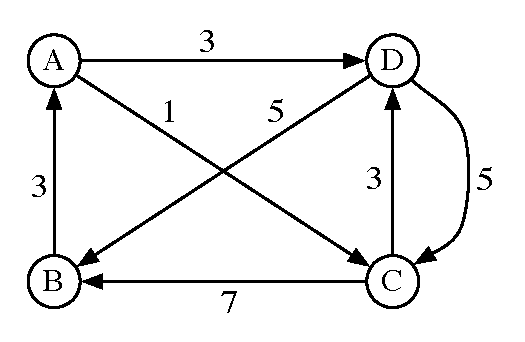
\includegraphics[width=2.5in]{amortized.pdf} %
\end{center}

Give a complete justification of your answer.

\paragraph{Answer}
We have the potential function: $\hat c_k = c_k + \Phi(D_k) - \Phi(D_{k-1})$. Suppose that the initial potentials of $A,\;B,\;C\;D\;$ are 0's, and we get $X$ after each step. To minimize $X$:\\
\begin{gather*}
    3 + D - A \leq X \\
    1 + C - A \leq X \\
    3 + A - B \leq X \\
    7 + B - C \leq X \\
    3 + D - C \leq X \\
    3 + B - D \leq X \\
    5 + C - D \leq X 
\end{gather*}
Then we can get the minimum possible value of $X$ is: $4$.

\end{problem}
%%%%%%%%%%%%%%%%%%%%%%%%%%%%

\vskip 0.3in
\paragraph{Submission.}
Submit the pdf file via gradescope by 5PM on Thursday, January 24.
For pair assignments, submit one pdf only with two names on it.

\vskip 0.3in
\paragraph{Challenge question.}
Suppose that a binary tree is only approximately
balanced. Does the formula
$\sum_{v\in T} \level(v) = O(n)$ still hold?
There are several ways to define what approximately
balanced is. For example,
(1) the tree has depth at most $C\log n$,
or
(2) for each node $x$, the heights of the left and right
        subtrees differ at most by $1$ (AVL tree),
or
(3) for each node $x$ with $m$ descendants, both its
        left and right descendant have at most $2m/3$
        descendants ($2/3$ is an arbitrary constant),
or
(4) the average depth in the tree is $O(\log n)$,
etc. For different definitions, the answers might be different.

\end{document}

